\documentclass[twocolumn]{article}
\usepackage{color}
\usepackage{cite}
\usepackage{draftwatermark}
\usepackage{multirow}
\usepackage{listings}
\usepackage{float}
\usepackage{amsfonts}
\usepackage{amssymb}
\usepackage{amsmath}
\usepackage{amsthm}
\usepackage{epsfig}
\usepackage{epstopdf}
\usepackage{titling}
\usepackage{url}
\usepackage{enumitem}
\usepackage{array}
\usepackage[utf8]{inputenc}
\usepackage[english]{babel}
\usepackage{tikz}
\usepackage{algorithm}
\usepackage[noend]{algpseudocode}
\usepackage{abstract}
\usepackage[inkscapeformat=png]{svg}


\usetikzlibrary{shapes,arrows,positioning,patterns,through}
\SetWatermarkText{Preview}
\SetWatermarkScale{1}
\setlength\parskip{.5\baselineskip}

\tikzset{
  dot node/.style={
    shape=circle,
    fill=white,
    draw,
    inner sep=+0pt,
    minimum size=+5mm
  },
  dotdot node/.style 2 args={
    dot node,
    label={[shape=circle,fill=black,outer sep=+0pt,inner sep=+0pt,minimum size=+3mm,name=ddd-#1,#2]center:}
  },
  arc style/.style={
    |<->|,
    shorten >=+-.5\pgflinewidth,
    shorten <=+-.5\pgflinewidth,
  }
}

\definecolor{pagecolor}{rgb}{0.9,1,1}
\pagecolor{pagecolor}


\author{
  Ryan J. Kung \\ ryankung@ieee.org
}
\title{The Ranking Protocol}

\begin{document}
\twocolumn[
  \begin{@twocolumnfalse}

\maketitle
\begin{abstract}
  This article presents a comprehensive reputation system for monitoring and evaluating the performance of nodes in a structured peer-to-peer (P2P) network. The system aims to foster responsible behavior and deter cheating among network participants.

The reputation system is comprised of two main components: local rankings and global rankings. Local rankings reflect the behavior of each node within its own network, while global rankings provide a comprehensive view of the behavior of all nodes in the entire network. To ensure the system's reliability, it utilizes reward proofs and punishment proofs. Nodes exhibiting good behavior are rewarded, while nodes engaging in undesirable actions are penalized, thus creating an environment where nodes are motivated to act ethically and cheating is discouraged.
  ~\\
  ~\\
\end{abstract}

\end{@twocolumnfalse}
]

\section{Introduction and Motivation}
The reputation system presented in this article aims to address the issue of monitoring node performance and preventing cheating in structured peer-to-peer (P2P) networks. By combining local and global rankings, the system provides a comprehensive evaluation of node behavior. The use of reward and punishment proofs incentivizes responsible behavior and discourages cheating, helping to maintain a healthy and secure network.

The system operates under the assumption of the Byzantine generals problem, where at least 2/3 of the nodes are assumed to be honest, as described in the literature \cite{time}. This helps to ensure the robustness and security of the network, allowing it to provide reliable and efficient services to users. Overall, the proposed reputation system represents a significant step forward in the development of secure and efficient structured P2P networks.

\subsection{Local Ranking}
The ranking protocol used in this system is inspired by Edonkey's Ranking Queue \cite{Edonkey}, and adopts a similar approach for monitoring node performance in the network. The objective is to prevent cheating, denial of service, and to maintain a healthy and secure network.

The system includes a mutual scoring system among nodes, which forms the basis of the measurement and local ranking system. The measurement system considers multiple metrics, such as the success rate of sent requests, the validity rate of received requests, and the total number of successful interactions. These metrics provide a comprehensive evaluation of a node's behavior and reliability.

By having each node maintain the scores of surrounding nodes independently, the system creates a decentralized and distributed local ranking system. This approach allows for a more accurate and comprehensive evaluation of node behavior and reliability, as it takes into account observations from multiple nodes in the network.

\subsection{Global Ranking}
The local rankings are used to generate the global ranking through a random sampling method. The random sampling method is based on a decentralized random number oracle, which ensures the fairness and impartiality of the global ranking. The use of a decentralized random number oracle helps to prevent any biases or manipulations in the ranking, ensuring that nodes are evaluated objectively and accurately.

The Ranking Protoocol implements the transformation from local ranking to global ranking through a four-phase random sampling procedure.

In the first phase, a random seed is generated to ensure the randomness of the sampling procedure and is typically generated by a decentralized oracle to eliminate centralization and bias.

In the second phase, the sampling targets are determined based on the local rankings and the random seed, using a systematic sampling algorithm.

In the third phase, the sample is selected from the local rankings based on the determined sampling targets, and a lookup algorithm is used to find the closest node to the target and provide proof of randomness using entropy test.

In the fourth phase, the validity of the sampling results is confirmed through a Kolmogorov-Smirnov (K-S) test to determine if the data is normally distributed. The K-S test compares the empirical cumulative distribution function of the data with the theoretical cumulative distribution function of the normal distribution, and returns a test statistic and a decision on the normality of the data.


\subsection{Reputation}

The ranking protocol uses the reputation system to incentivize and ensure fair local and global rankings. The global ranking is generated through fair random sampling of the local ranking.

The reputation system rewards nodes for good behavior and punishes nodes for bad behavior. This helps to incentivize nodes to behave properly and discourage cheating. The reputation system is designed to maintain a healthy and robust network by promoting fair and honest behavior among nodes.

\section{Related Work}

The edonkey Ranking Queue is a well-known mechanism in the peer-to-peer network community for evaluating node performance. The Rings network adopts a similar approach to the edonkey Ranking Queue to implement its local ranking system.

One relevant work is the eDonkey network, which uses the edonkey Ranking Queue as its mechanism for monitoring node performance. The eDonkey network was one of the earliest peer-to-peer networks to use a mutual scoring system among nodes to prevent cheating or denial of service.

Another related work is the Bittorrent network, which utilizes a mechanism called "choking" to prevent cheating or denial of service. The Bittorrent network evaluates node performance based on the speed and reliability of data transfers, and nodes that perform poorly are restricted from receiving data from other nodes.

In conclusion, the ranking protocol used in the Rings network draws inspiration from the edonkey Ranking Queue and other related works in the peer-to-peer network field. By using a mutual scoring system among nodes, the Rings network aims to provide a secure and efficient peer-to-peer network that can accurately evaluate node performance and prevent cheating or denial of service.

\section{Sampling}

The Ranking Protoocol effectuates a transformation from local ranking to global ranking through a random sampling procedure, which can be decomposed into four phases:

\textbf{1. Generation of a random seed:}

A random seed is generated to guarantee the randomness of the sampling procedure. The random seed is typically generated through a decentralized oracle to ensure a lack of centralization and bias in the generation process.

\textbf{2. Determination of sampling targets:} Sampling targets are determined based on the local rankings and the randomly generated seed.

\begin{algorithm}[htbp]
  \caption{Systematic Sampling}
  \label{samping}
\begin{algorithmic}[1]
\State $K \gets \lfloor \frac{2^n}{2^m} \rfloor$
\State $r \gets$ random number between 0 and 1
\State $s \gets \lfloor K \cdot r \rfloor$
\State Select elements at positions $s, s + K, s + 2K, \dots$
\end{algorithmic}
\end{algorithm}

We use simple Systematic samping algorithm \ref{samping} here, where n is the number of bits in the random number and m is the desired range of the random sample. The final result is a systematic sample of elements within the range (0, $2^m$).

\textbf{3. Sampling process:} The elements in the local ranking are selected as a sample based on the determined sampling targets.

\begin{algorithm}[htbp]
\begin{algorithmic}[1]
\Require{Data sequence $S$}
\Ensure{Whether the input data is random or not}
\State Calculate the frequency $f_i$ of each character in $S$
\State Calculate the entropy $H(S)$ using Shannon entropy or Renyi entropy formula
\State Calculate the expected entropy $H_{exp}$ based on the length of $S$ and the size of the character set
\If{$|H(S)-H_{exp}|<\epsilon$}
\State \Return{True}
\Else
\State \Return{False}
\EndIf
\end{algorithmic}
\label{entropy}
\caption{Entropy Testing Algorithm}
\end{algorithm}



Due to the potentially large number of nodes in a DHT\cite{Chord} network, it may not be possible to exactly locate the target in the sample processing stage. As a result, the sample processing becomes an approximation process, where the DHT network uses a lookup algorithm to find the peer closest to the sample target and provides proof of proximity.

This is because for most DHT implementations, such as KAD and Chord, it is impossible to have random ID collisions. Therefore, during the sampling process, the triggered lookup protocol can only get as close as possible to the sampled position. For our $[r_i,.., r_n]$ random numbers, we will obtain $[(id_i, r_i, .., id_n, r_n)]$ through the DHT lookup algorithm. At this point, we will use entropy testing \ref{entropy} to prove that the distance difference $\Delta_i$ between the sampled nodes and the sampling target has randomness, where $\Delta_i = did_i - r_i$.

\textbf{4. Validation of sampling results:} The sampling results are validated to confirm their representativeness of the true order of elements in the queue.

We use Kolmogorov-Smirnov(K-S) test to check the result data of sampling is normally distributed. The KS test works by comparing the empirical cumulative distribution function (CDF) of the data with the theoretical CDF of the normal distribution. K-S is described as:
Let $F_{n}(x)$ be the empirical cumulative distribution function (CDF) of a sample of size $n$, and let $F(x)$ be the theoretical CDF of the normal distribution. The Kolmogorov-Smirnov test statistic is defined as:

\begin{equation}
D = \sup_{x} \left| F_{n}(x) - F(x) \right|
\end{equation}

where $\sup$ represents the supremum, or the least upper bound. The value of $D$ measures the maximum difference between the empirical and theoretical CDFs, and is used to determine whether the data is normally distributed.

The null hypothesis of the KS test is that the data is normally distributed, and the alternative hypothesis is that the data is not normally distributed. The test statistic $D$ is compared to critical values from the KS distribution to determine whether to reject or fail to reject the null hypothesis. If the test statistic is greater than the critical value, the null hypothesis is rejected, and the data is considered not to be normally distributed.


\begin{algorithm}[htbp]
\caption{Kolmogorov-Smirnov Test}
\begin{algorithmic}[1]
\State \textbf{Input:} Sample data $x_1, x_2, \dots, x_n$
\State \textbf{Output:} Test statistic $D$ and decision on normality of data

\State Calculate the empirical cumulative distribution function (CDF) $F_{n}(x)$ for the sample data
\State Calculate the theoretical cumulative distribution function (CDF) $F(x)$ for the normal distribution
\State Calculate the test statistic $D$ using the formula:
\begin{equation}
D = \sup_{x} \left| F_{n}(x) - F(x) \right|
\end{equation}
\State Compare the test statistic $D$ to critical values from the KS distribution
\If{$D \leq critical_value$}
\State \textbf{return} "Data is normally distributed", $D$
\Else
\State \textbf{return} "Data is not normally distributed", $D$
\EndIf
\end{algorithmic}
\label{ks}
\end{algorithm}

And the algorithm can be present as \textbf{algorithm \ref{ks}}.

This algorithm calculates the empirical and theoretical CDFs for the sample data and the normal distribution, and calculates the test statistic $D$ as the maximum difference between the empirical and theoretical CDFs. The test statistic is then compared to critical values from the KS distribution to determine whether the data is normally distributed or not. The algorithm returns the test statistic and a decision on the normality of the data.


\section{Ranking game}


For the sampled nodes, we need to introduce a reward mechanism to encourage them to be honest. We will use the median of the sampling results and reward the nodes closest to the median. This will introduce a series of games, and we will analyze them from multiple aspects, including the median game, the complete information game, the incomplete information game, and the game based on the Byzantine generals problem.

\subsection{Guess the Median}

We use a Guess the Median\cite{game_theory} method to build a game between the sampled nodes, for the sampled objects, the sampled nodes need to have enough motivation to participate, which means rewards, but also means the possibility of cheating. Therefore, we only reward nodes that are close to the Median.

In this game, each player has two strategies: to guess a number that is higher than the median, or to guess a number that is lower than the median. Let's denote the strategy of guessing a number that is higher than the median as H, and the strategy of guessing a number that is lower than the median as L.

The game matrix for Guess the Median would then look like this:

\begin{figure}[htbp]
  \begin{center}
    \begin{tabular}{c|cc} & H & L \\ \hline H & R & S \\ L & T & P \\ \end{tabular}
  \end{center}

\caption{Two player median}
\end{figure}

where R is the reward for both players guessing higher than the median, S is the cost for one player guessing higher and the other guessing lower, T is the cost for both players guessing lower than the median, and P is the reward for one player guessing higher and the other guessing lower.

In this game, the median is considered the Nash Equilibrium, meaning that neither player has an incentive to deviate from their current strategy as long as the other player stays the same. This ensures that both players are motivated to participate and incentivizes honest behavior.

This game can be applied to the nodes in the network to incentivize honest and accurate reporting of their local rankings. The nodes that accurately report their rankings and are close to the median will be rewarded, while nodes that cheat or deviate from the correct rankings will be penalized.

\subsection{Complete Information game}
When nodes need to decide whether to be honest during sampling, this problem can be simplified into a complete information game. In a complete information game, each player has complete information, including the strategy choices and payoff functions of other players. Therefore, each node knows whether other nodes are behaving honestly during the sampling process, as well as the rewards and payoffs of other nodes.

Assuming that each player can only choose one of two strategies, "Be honset" (X) or "not be honest" (Y), and the payoffs are as follows:

\begin{figure}[htbp]
\begin{tabular}{c|cc}
& \textbf{Player C X} & \textbf{Player C Y} \\
\hline
\textbf{Player A} & (1,1,1) & (0,0,1) \\
\textbf{Player B} & (1,1,1) & (0,0,1) \\
\textbf{Player C} & (1,1,1) & (1,0,1) \\
\end{tabular}
\end{figure}

In this matrix, the first number in each cell represents the payoff for Player A, the second number represents the payoff for Player B, and the third number represents the payoff for Player C. For example, if all three players choose strategy X, then each player will get a payoff of 1, as indicated in the top left cell.

If all players choose H, each player gets a payoff of 1. If two players choose H and one player chooses C, the two players who choose H get a payoff of 1, while the player who chooses C gets a payoff of 0. If all players choose C, each player gets a payoff of 1.

In this game, there are two pure strategy Nash equilibria, which are (X, X, X) and (Y, Y, Y). If all players choose to either reveal or conceal the information, then none of them can improve their payoff by changing their strategy. In addition, there is a mixed strategy Nash equilibrium in which each player randomly chooses the two strategies with equal probability, which results in each player getting an expected payoff of 2/3.

It's worth noting that the payoffs for all players are the same in both pure strategy Nash equilibria, and each player gets a higher payoff than in the mixed strategy Nash equilibrium. However, the mixed strategy Nash equilibrium is also a valid solution concept in game theory, and it may be a more realistic description of what happens when the players are uncertain about each other's strategies or preferences.


\subsection{Bayesian game}

In the game above, we assumed that the information was complete, and each node knew how others would act, so the outcome of the game was that they would either all choose honestly or all cheat, which is similar to the Byzantine Generals Problem. In fact, the game process could also be an incomplete information game, which is a Bayesian game, where each node is uncertain about whether the other nodes know information I.

If each player does not know which strategy the other players have chosen, the game becomes an asymmetric information game, also known as a Bayesian game. In this case, we can use an extended game matrix to represent each player's strategies and possible payoffs.

To simplify the problem, let's assume that each player knows information I, but does not know whether the other players know this information. In this case, each player has two information sets: knowing information I and not knowing information I. Each information set has two strategies: showing information I and hiding information I. Therefore, each player has four possible strategy combinations.

\begin{figure}[H]
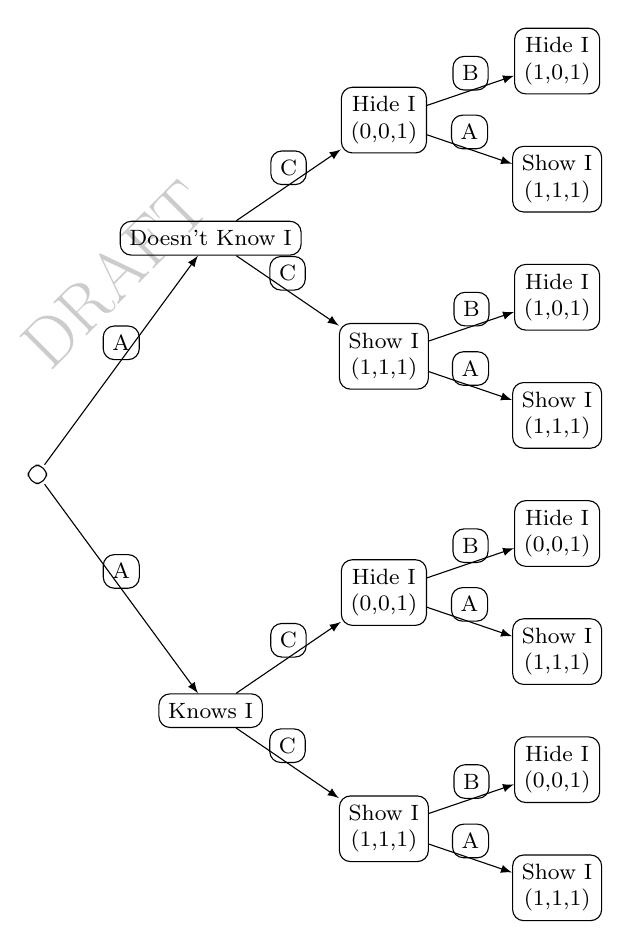
\begin{tikzpicture}[  level distance=2.2cm,  level 1/.style={sibling distance=6cm},  level 2/.style={sibling distance=3cm},  level 3/.style={sibling distance=1.5cm},  grow=right,  font=\footnotesize,  edge from parent/.style={draw,-latex},  every node/.style={draw, rounded corners, align=center},  ]

  \node {}
  child {
    node {Knows I}
    child {
      node {Show I \\ (1,1,1)}
      child {
        node {Show I \\ (1,1,1)}
        edge from parent node[above] {A}
      }
      child {
        node {Hide I \\ (0,0,1)}
        edge from parent node[above] {B}
      }
      edge from parent node[above] {C}
    }
    child {
      node {Hide I \\ (0,0,1)}
      child {
        node {Show I \\ (1,1,1)}
        edge from parent node[above] {A}
      }
      child {
        node {Hide I \\ (0,0,1)}
        edge from parent node[above] {B}
      }
      edge from parent node[above] {C}
    }
    edge from parent node[above] {A}
  }
  child {
    node {Doesn't Know I}
    child {
      node {Show I \\ (1,1,1)}
      child {
        node {Show I \\ (1,1,1)}
        edge from parent node[above] {A}
      }
      child {
        node {Hide I \\ (1,0,1)}
        edge from parent node[above] {B}
      }
      edge from parent node[above] {C}
    }
    child {
      node {Hide I \\ (0,0,1)}
      child {
        node {Show I \\ (1,1,1)}
        edge from parent node[above] {A}
      }
      child {
        node {Hide I \\ (1,0,1)}
        edge from parent node[above] {B}
      }
      edge from parent node[above] {C}
    }
    edge from parent node[above] {A}
  };
\end{tikzpicture}
\caption{Bayesian Game}
\label{bayes}
\end{figure}

To represent each player's possible payoffs, we can use a set of tree diagrams, where each node represents a possible decision point, each edge represents a player's decision, and each leaf node represents each player's possible payoff. In this context, we can draw the following game tree:

In this game tree \ref{bayes}, each player has two information sets represented by circles. Each information set has two strategies represented by squares. Each leaf node represents each player's possible payoff, where the first number represents Player A's payoff, the second number represents Player B's payoff, and the third number represents Player C's payoff. For example, if Player A chooses to show information I while Player B and Player C both choose to hide information I, then Player A's payoff is 0, while Player B and Player C both receive a payoff of 1.

\begin{figure}[htbp]
\begin{tabular}{c|cc}
& Show I & Hide I \\
\hline
Show I & 1, 1, 1 & 0, 1, 1 \\
Hide I & 1, 0, 1 & 1, 1, 0 \\
Show I & 1, 1, 1 & 0, 1, 1 \\
  Hide I & 1, 0, 1 & 1, 1, 0 \\
\end{tabular}
  \label{bayes mat}
  \caption{Bayesian Game Matrix}
\end{figure}


The game can also be represented using a game matrix as \ref{bayes mat}. In this matrix, each row and column represents a player's strategy, and the numbers in each cell represent the payoffs for the three players. The first row and first column correspond to player A's strategy choices, the second row and column correspond to player B's strategy choices, and the third row and column correspond to player C's strategy choices.

There are two Nash equilibria in this game: (Show I, Show I, Show I) and (Hide I, Hide I, Hide I). In the first Nash equilibrium, all players reveal the information since this is the only choice that results in the maximum payoff for all players. In the second Nash equilibrium, all players keep the information hidden since revealing it would result in a loss for the player who does not reveal it.

\subsection{Distributed Game}
If we assume that 2/3 of the players are honest, then the game becomes a variant of the Majority-vote game. This game has been extensively studied in the field of distributed computing and fault tolerance, where it is used as a model for solving consensus problems in distributed systems. In this game, each player can choose to vote for one of two options, and the goal is to determine the majority vote.

The Byzantine Generals' Problem is a specific instance of the Majority-vote game, where some players may be malicious or faulty and try to manipulate the outcome of the game. In this variant of the game, the players may have different beliefs about the number of honest players, and this may affect their strategies.

If we assume that 2/3 of the people are honest, then each player may assume that the other players are honest with a probability of 2/3, which is a reasonable assumption. Based on this assumption, each player may be more inclined to reveal the information I, as it is the optimal strategy for all players and the other players may also choose to reveal the information.

However, each player's optimal strategy will also depend on their level of trust in the other players. If a player believes that the other players are not sufficiently honest, they may be more inclined to keep the information I hidden to avoid being deceived or harmed by the other players. Therefore, the players' strategies will depend on their beliefs about the other players' strategies, and whether they think the other players are likely to reveal the information or keep it hidden.

\begin{figure}[htbp]
  \begin{center}
\begin{tabular}{c|cc}
& A chooses X & A chooses Y \\
\hline
B chooses X & $(\frac{4}{9}, \frac{4}{9}, \frac{4}{9})$ & $(\frac{1}{9}, \frac{1}{9}, \frac{1}{9})$ \\
B chooses Y & $(\frac{1}{9}, \frac{1}{3}, 0)$ & $(\frac{2}{9}, \frac{2}{9}, 0)$ \\
\end{tabular}
\end{center}
\label{dgame}
\caption{Distributed game}
\end{figure}

The game matrix for this game would look like this \ref{dgame}, each row and column represents a player's strategy, and the numbers in each cell represent the payoffs for the three players. The first row and first column correspond to player A's strategy choices, the second row and column correspond to player B's strategy choices, and the third row and column correspond to player C's strategy choices.

For this distributed game, we need to find the best responses for each player and then determine if there exists a Nash equilibrium solution.

First, we consider the best response for player B. If player A chooses X, then the best response for player B is to choose X, because $(\frac{4}{9}, \frac{4}{9}, \frac{4}{9})$ is better than $(\frac{1}{9}, \frac{1}{3}, 0)$. If player A chooses Y, then the best response for player B is to choose Y, because $(\frac{2}{9}, \frac{2}{9}, 0)$ is better than $(\frac{1}{9}, \frac{1}{9}, \frac{1}{9})$. Therefore, player B will choose the same strategy as player A.

Next, we consider the best response for player A. If player B chooses X, then the best response for player A is to choose X, because $(\frac{4}{9}, \frac{4}{9}, \frac{4}{9})$ is better than $(\frac{1}{9}, \frac{1}{9}, \frac{1}{9})$. If player B chooses Y, then the best response for player A is to choose Y, because $(\frac{2}{9}, \frac{2}{9}, 0)$ is better than $(\frac{1}{9}, \frac{1}{3}, 0)$. Therefore, player A will also choose the same strategy as player B.

Therefore, In this game, due to the consideration of the Byzantine assumption, the unique Nash equilibrium solution is when player A and player B both choose X, which corresponds to a payoff of $(\frac{4}{9}, \frac{4}{9}, \frac{4}{9})$, that all nodes will tend to remain honest.


\subsection{Rank maximize}


Let's consider the scenario where individuals are able to repeatedly calculate their global rank until they are satisfied with the outcome. This raises two questions: 1) Will the repeated sampling by the sampler result in a significant increase in network traffic, and 2) Will the sampled individuals be willing to disclose their accurate local rank.

To optimize the results of the sampling process, the sampler must consider the normal distribution generated by the ranking protocol. As the number of requests made by nodes increases, the maximum value of the normal distribution may decrease. To achieve the highest result possible, the sampler must adjust the number and timing of samplings based on a thorough understanding of the normal distribution.

To determine the most optimal strategy, statistical analysis of the mean and variance of the normal distribution is necessary. This allows the sampler to evaluate different strategies and choose the one that will provide the best results. By performing this analysis, the sampler can optimize the results of the sampling process and achieve the most accurate global ranking.

\begin{align}
  \max_x \quad & n \\
  \text{subject to} \quad & g_i(x) \leq 0, \quad i = 1, \dots, m \\
  & h_j(x) = 0, \quad j = 1, \dots, p
\end{align}

In this model, x is a vector of variables that represent the actions taken by A, n is the objective function to be maximized, $g_i(x)$ represents the inequality constraints, and $h_j(x)$ represents the equality constraints. The goal is to find the values of x that maximize n subject to the constraints.


\subsection{Sample weight}
Once nodes obtain the Global Rank, we can calculate their weight based on the Global Rank of the sampled nodes during the sampling process, with higher Global Rank of the sampled objects having a higher weight.

To handle the network's cold start problem, initially, all Global Ranks are set to 0. In order to jumpstart the ranking process, a set of initial high-ranking nodes are introduced to facilitate credit transfer. These nodes are assigned a high Global Rank and their ranking is used as a reference for other nodes to calculate their own Global Rank in subsequent samples. This allows for a gradual increase in the Global Rank of other nodes as they participate in the sampling process and receive rewards based on their proximity to the median.
\subsection{Reward and Slash Proofs}

This way, the system can have both financial incentives and deterrents to maintain the accuracy and reliability of the rankings. The locking mechanism also helps to prevent malicious behavior and cheating, as nodes would have to consider the consequences of their actions before participating in the ranking system. The use of cryptographic signatures and the distributed ledger further enhances the security and transparency of the system. Overall, the combination of rewards, punishments, and locking mechanisms creates a balanced system that incentivizes nodes to contribute to the accuracy and reliability of the ranking system while also deterring malicious behavior.

\section{Economics}

It is generally desirable for Rankings to deflate, as this increases their value. To achieve this, the Rankings need to be made payable, allowing users to use them to purchase services or participate in liquidity staking.

As Sampling continues, the average value of the network's Rankings will increase and the total supply of Rankings will become larger, causing the unit value of Rankings to decrease. To counteract this, the supply within a single Sample Round should be fixed, requiring the results of Sampling to be revealed at a later time. Participants can estimate the quality of their Sample results, but cannot determine their specific value. With a fixed supply, the growth of Rankings becomes linear. As the network grows, obtaining high Rankings becomes more difficult, and so it is suggested that the supply should have a positive correlation with the network size. This means that for each Sample Round, the number of participating nodes $n_i$ and the total supply $s_i$ are established. When $n_i > n_{i-1}$, $s_i$ should be greater than $s_{i-1}$.

\begin{figure}[htbp]
  \label{supply}
\begin{align}
  S_i &= \sum_{i=0}^{i}knc_i\\
  \Delta S &= S_i - S_{i-1} = knc_i\\
  \Delta V &= \frac{knc_i}{S}
 \end{align}
\end{figure}

The figure \ref{supply} illustrates the alteration of the total supply and the value of the token.

And to realize deflation, it is necessary to make the Ranking payable, which typically implies that users are able to utilize it to purchase services or participate in liquidity staking.

Another approach to achieve deflation is to periodically halve the fixed supply of Rankings, similar to how Bitcoin operates. This method ensures a controlled and predictable reduction in the overall supply of Rankings, thereby increasing its unit value over time.


\section{Conclusion}
Overall, the Ranking Protoocol provides a comprehensive and effective solution for evaluating node performance and preventing cheating or denial of service in structured peer-to-peer networks. By using a mutual scoring system among nodes and a reputation system that incentivizes proper behavior, the Ranking Protoocol aims to provide a secure and efficient peer-to-peer network.
\bibliographystyle{unsrt}
\bibliography{./cites}
\end{document}